%!TEX root=./robocert.tex
%
% RoboCert Graphical notation (using TikZ)
%
% Last updated: 2022-08-26
%

\newcommand{\rckeywordfont}{\sffamily\bfseries}
\newcommand{\rckeyword}[1]{{\rckeywordfont #1}}
\newcommand{\rcosigil}{\rckeyword{op}}
\newcommand{\rcesigil}{\rckeyword{event}}

\newlength{\rctopmargin}
\setlength{\rctopmargin}{3em}

\newlength{\rcstepmargin}
\setlength{\rcstepmargin}{.2em}

% Shading used for various parts of the graphical notation.
% Colour to be used very sparingly here.
\colorlet{rcshading}{black!20}

\usetikzlibrary{arrows.meta,matrix,shapes,calc,fit}
\tikzset{
    rcseq/.style={row sep=2.2em, column sep=8em},
% Actors
    rcactor/.style={draw, rectangle, minimum width=4em, align=center, minimum height=1.7em, fill={rcshading}, font={\footnotesize\sffamily}},
% Control flow
    rclifeline/.style={thick},
    cfbox/.style={draw, solid},
    cfheader/.style={chamfered rectangle, draw, font={\scriptsize\sffamily}, fill={rcshading}, chamfered rectangle corners=south east, inner sep=0.1em},
    branchdiv/.style={draw, thick, dotted},
    guard/.style={font={\scriptsize\sffamily}, anchor=north east, align=right, inner sep=0.2em},
% Deadlines
    deadline/.style={solid, font={\scriptsize}},
    deadlinespan/.style={latex-latex},
% Temperature modalities
    cold/.style={thick, solid},
    hot/.style={cold, double},
% Occurrences
    arrow/.style={->, cold},
    arrowlabel/.style={fill=white, font={\scriptsize\sffamily}, inner sep=0.2em},
    wait/.style={cold, font={\scriptsize}},
    end/.style={fill, very thick, rectangle, minimum height=3pt, minimum width=15pt, inner sep=0em}
}

% pseudo-UML stereotype name
% #1: name of the stereotype
\newcommand{\rcstereotype}[1]{\rckeyword{\(\langle\!\langle\)\,#1\,\(\rangle\!\rangle\)}}

% Target actor
\newcommand{\rctarget}{\rcstereotype{target}}

% Component actor
% #1: name of the type
\newcommand{\rccomponent}[1]{\rcstereotype{component} #1}

\newcommand{\gdiff}[2]{#1\setminus#2}
\newcommand{\guniverse}{\ast}
\newcommand{\gextset}[1]{\{#1\}}
\newcommand{\gemptyset}{\gextset{}}
\newcommand{\grefset}[1]{\textsf{#1}}

% Header for sequence diagrams
%
% #1: name of diagram
% #2: name of target
\newcommand{\rcseq}[2]{\rckeyword{sd} #1 (#2)}

% Combined fragment or diagram frame
% #1: padding factor
% #2: top-left
% #3: bottom-right
% #4: header
\newcommand{\rcframe}[4]{
  % Slightly eccentric definition here to line the world up with the RHS,
  % and leave room for the top 'sd' line.
  \draw ($(#2) + (-#1*\the\rcstepmargin, \the\rctopmargin)$) rectangle ($(#3) + (#1*\the\rcstepmargin, -#1*\the\rcstepmargin)$);
  \node[cfheader, anchor=north west] at ($(#2) + (-#1*\the\rcstepmargin, \the\rctopmargin)$) {\footnotesize #4};
}

% Guard
% #1: name
% #2: position (right edge of box)
% #3: expression
\NewDocumentCommand{\gguard}{m m m}{\node[guard] (#1) at (#2) {[#3]};}

% Wildcard with an optional binding
\NewDocumentCommand{\gwildcard}{o}{\rckeyword{any}\IfValueT{#1}{ \rckeyword{as} #1}}
\NewDocumentCommand{\gusebinding}{m}{\rckeyword{@}#1}

% The 'otherwise' guard
\NewDocumentCommand{\gotherwise}{}{otherwise}

% Loop
% #1: coordinates to fit
% #2: loop name
% #3: loop header
% (#4: inner sep)
% (#5: horizontal inner sep)
\NewDocumentCommand{\gloop}{m m m O{0.4em} O{0}}{\gcfrag{#1}{#4}{\rckeyword{loop}#3 #2}{loop#2}[cfbox][#5]}

% Gap
% #1: top-left
% #2: name
% #3: set
% (#4: inner sep)
% (#5: horizontal inner sep)
\NewDocumentCommand{\guntil}{m m m O{0.3em} O{1.1em}}{\gcfrag{#1}{#4}{\rckeyword{any}(\(#3\)) \rckeyword{until} }{#2}[cfbox][#5]}

% Branch division
% #1: name of branch
% #2: right
\NewDocumentCommand{\gbranchdiv}{m m}{
  \draw (#2 -| brbranch#1)
        edge[branchdiv]
        (#2 -| branch#1.west)
  ;
}

% Branch
% #1: fit
% #2: branch name
% #3: branch header
\NewDocumentCommand{\gbranch}{m m m}{\gcfrag{#1}{0.1em}{#3 #2}{branch#2}}

% Alternative branch header
\NewDocumentCommand{\galternative}{}{\rckeyword{alt}}
% X-Alternative branch header
\NewDocumentCommand{\gxalternative}{}{\rckeyword{xalt}}
% Parallel branch header
\NewDocumentCommand{\gparallel}{}{\rckeyword{par}}
% Optional block header
\NewDocumentCommand{\gopt}{}{\rckeyword{opt}}


% Loop bounds
% These follow UML for now.
\newcommand{\gloopinfinite}{}
\newcommand{\gloopdefinite}[1]{(#1)}
\newcommand{\glooprange}[2]{(#1, #2)}
\newcommand{\glooplower}[1]{\glooprange{#1}{\(\ast\)}}

% Generic message command
% #1: LHS
% #2: RHS
% #3: sigil
% #4: label
% #5: temperature
\NewDocumentCommand{\gmessage}{m m m m m}{\draw (#1) edge[arrow, \IfBooleanTF{#5}{hot}{cold}] node[arrowlabel] {#3\(\;\)#4} (#2);}

% #1: temperature (star)
% #2: LHS
% #3: RHS
% #4: label
% #5: argument(s)
\NewDocumentCommand{\goperation}{s m m m m}{\gmessage{#2}{#3}{\osigil}{#4(#5)}{#1}}

% #1: temperature (star)
% #2: LHS
% #3: RHS
% #4: label
% #5: return value (optional)
\NewDocumentCommand{\gevent}{s m m m o}{\gmessage{#2}{#3}{\esigil}{#4\IfValueT{#5}{(#5)}}{#1}}

% #1: temperature (star)
% #2: LHS
% #3: RHS
% #4: units expression
\NewDocumentCommand{\gwait}{s m m m}{\draw (#2) edge[wait, \IfBooleanTF{#1}{hot}{cold}] node[arrowlabel] {\rckeyword{wait}(#4)} (#3);}

\newcommand{\gdeadlinehoffset}{0.6em}
\newcommand{\gdeadlinevoffset}{0.5em}
% #1: Top
% #2: Bottom
% #3: Bounds set
% #4: Lower bound
\NewDocumentCommand{\gdeadline}{m m m}{
  \draw[deadline]
    ($(#1) + (0, \gdeadlinevoffset)$)
      --
    ($(#1) + (-\gdeadlinehoffset, \gdeadlinevoffset)$);
  \draw
    ($(#2) + (-\gdeadlinehoffset, -\gdeadlinevoffset)$)
      edge[deadlinespan] node[font=\scriptsize, anchor=east, inner sep=0.2em] {#3}
    ($(#1) + (-\gdeadlinehoffset, \gdeadlinevoffset)$)
      edge[deadline]
    ($(#2) + (0, -\gdeadlinevoffset)$);
}

We define \langname{} as a formal abstract syntax (or
metamodel) which is representable in multiple concrete notations ---
the \emph{textual} (\cref{cha:textual}) and \emph{graphical}
syntax (\cref{cha:graphical}) --- and which has a semantics in terms
of process algebras and other formalisms (\cref{cha:semantics}).  This
chapter discusses the abstract syntax and, in turn, the key concepts
of \langname.

\section{Introduction}\label{sec:metamodel-intro}

\subsection{A note on ordering and timing}\label{ssec:metamodel-intro-ordering}

By default, \langname{} sequences are \emph{explicit}
as to \emph{which} actions occur, but \emph{implicit} as to
\emph{when}.

Unless modified by gaps (\cref{ssec:metamodel-steps-gaps}),
communications on \langname{} sequences are strictly ordered with
respect to each other and permit no intervening communications.  This
reflects the view of sequence diagrams as representations of traces of
the system under test, and appears consistent with some semantic
treatments of UML~\cite{lima-semantics}.  \todo{needs more
  justification?  is the point about Lima's semantics correct?}

\langname{} uses the \robochart{} timing model, and some \robochart{}
timing primitives have direct counterparts in \langname.  This model
assumes a discrete notion of time measured in \emph{time units} such
that, while actions such as events and operations are instantaneous,
time is allowed to pass in between them.  We take the approach of
assuming that where time can pass in the \robochart{} model,
\emph{any} amount of time may pass in the sequence, unless
constrained by deadlines (\cref{ssec:metamodel-steps-deadlines}).


\subsection{How to read the rest of this chapter}\label{ssec:metamodel-intro-readme}

Each section, except this one and \cref{sec:metamodel-features},
introduces a group of related \langname{}
functionality in a top-down manner.  These sections contain:

\begin{itemize}
\item
	a class diagram representing the Ecore classes, enumerations, and other
	components that make up the group being discussed;
\item
	descriptions of the components being shown in the class diagram;
\item
	where relevant, examples of the components in terms of the concrete
	syntaxes of \langname.
\end{itemize}

\section{Top}\label{sec:metamodel-top}
% !TEX root=../../robocert.tex
\begin{figure}[htb]
  \centering
  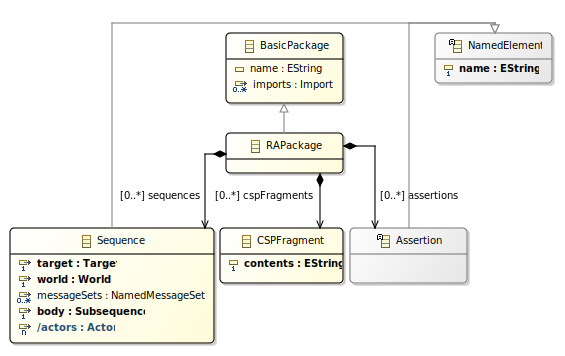
\includegraphics[width=.85\textwidth]{diagrams/Top}
  \caption{Class diagram for the top of the \langname{} metamodel.}
  \label{fig:metamodel-top}
\end{figure}

\Cref{fig:metamodel-top} is the top-level metamodel diagram for \langname.

Each \langname{} script contains an \mrapackage,\footnote{\mrapackage{} stands
  for `RoboStar Assertions package'; we use this name because \mrcpackage{} is
  already used for RoboChart packages.}
which is a type of RoboStar \mbasicpackage.
Each \mrapackage{} can contain zero or more of each of these types of content:

\begin{itemize}
\item
  \msequencegroup:
  a sequence diagram group
  (see \cref{sec:metamodel-sequences});
\item
  \mcspfragment:
  a CSP fragment, currently not bound to a particular process
  \todo{this will change};
\item
  \massertion:
  an assertion
  (see \cref{sec:core-metamodel-assertions}).
\end{itemize}

%%% Local Variables:
%%% mode: latex
%%% TeX-master: "../../robocert"
%%% End:


\section{Sequences}\label{sec:metamodel-sequences}
%!TEX root=../robocert.tex
\begin{figure}[htb]
	\centering
	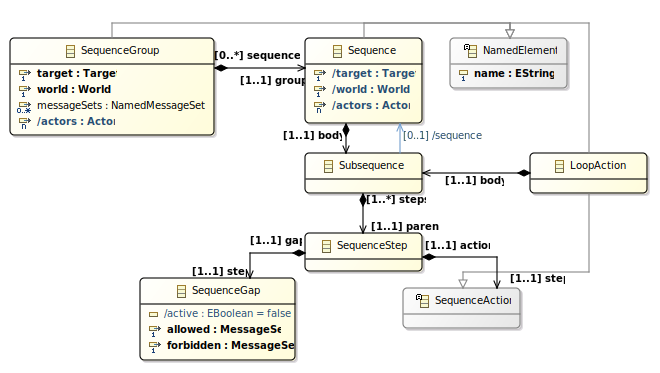
\includegraphics[width=\textwidth]{diagrams/Sequences}
	\caption{Class diagram for the part of the \langname{} metamodel dealing with sequences.}
	\label{fig:metamodel-sequences}
\end{figure}

The main tool for specifying properties of \robochart{} models in
\langname{} is \emph{sequences}.  These are diagrams, similar to UML2
sequence diagrams~\cite{lima-semantics} and Property Sequence Charts~\cite{psc},
that capture one or more valid traces of a robotic system.

\Cref{fig:metamodel-sequences} depicts the part of the metamodel concerning
sequence groups and sequences.

\subsection{\msequencegroup}

A \msequencegroup{} is a top-level \mnamedelement{} that contains sequence diagrams.
It contains:

\begin{itemize}
\item
  two \mactor s (\cref{sec:metamodel-actors}):
  a \mtarget{} (\cref{ssec:metamodel-actors-target})
  and a \mworld{} (\cref{ssec:metamodel-actors-world});
\item
  zero or more \mnamedmessageset{}s (\cref{ssec:metamodel-messages-named-sets});
\item
  zero or more \msequence{} (\cref{ssec:metamodel-sequences-sequences}).
\end{itemize}

\begin{lstlisting}[style=Example]
sequence group Group:
  module AModule  // RCModuleTarget actor
  -> world        // World actor
{
  message set M1: universe
  
  sequence Example1 {
    anything until end
  }
  sequence Example2 {
    anything until end
  }
}
\end{lstlisting}

\subsection{\msequence}\label{ssec:metamodel-sequences-sequences}

A \msequence{} represents a sequence diagram.  It is a \mnamedelement{}
that contains a \msubsequence{} (\cref{ssec:metamodel-sequences-subsequences})
capturing the body of the diagram.

\begin{figure}[h!]

  \begin{subfigure}[t]{\egtextwidth}
    \begin{lstlisting}[style=Example]
sequence Example {
  anything until end  // Subsequence
}
    \end{lstlisting}
  \end{subfigure}
  \hfill
  \begin{subfigure}[t]{\eggraphicalwidth}
    \gsecaption
    \centering
    \begin{tikzpicture}
      \matrix[diagram]{
        \node[rcmodule](mstart) {\egtarget}; & \node[world](wstart) {\egworld}; \\
	\coordinate(mend); & \coordinate(wend); \\
      };
      \gseq{wstart}{mstart}{wend}{mend}{Example}
      \draw[lifeline] (wstart) -- (wend);
      \draw[lifeline] (mstart) -- (mend);
      \gfinal{mend}{wend}
      \ggapout{mend}{\guniverse}
    \end{tikzpicture}
  \end{subfigure}

\end{figure}

\subsection{\msubsequence}\label{ssec:metamodel-sequences-subsequences}

A \msubsequence{} is a sequential composition of one or more \msequencestep s
(\cref{sec:metamodel-steps}).
All \msequence s contain exactly one \msubsequence{} at the top level, but
may contain multiple nested \msubsequence s introduced by control-flow
\msequencestep s.

\begin{figure}[h!]

  \begin{subfigure}[t]{\egtextwidth}
    \begin{lstlisting}[style=Example]
{
  anything until ->op O1() // SequenceStep
  then           ->op O2() // SequenceStep
  then end                 // SequenceStep
}
    \end{lstlisting}
  \end{subfigure}
  \hfill
  \begin{subfigure}[t]{\eggraphicalwidth}
    \gsecaption
    \centering
    \begin{tikzpicture}
      \matrix[diagram]{
        \node[rcmodule](mstart) {\egtarget}; & \node[world](wstart) {\egworld}; \\
	\coordinate(mo1); & \coordinate(wo1); \\
	\coordinate(mo2); & \coordinate(wo2); \\
	\coordinate(mend); & \coordinate(wend); \\
      };

      \draw[lifeline] (mstart) -- (mo1) -- (mo2) -- (mend);
      \draw[lifeline] (wstart) -- (wo1) -- (wo2) -- (wend);

      \goperation{mo1}{wo1}{O1()}
      \ggapout{mo1}{\guniverse}
      \goperation{mo2}{wo2}{O2()}
      
      \gfinal{mend}{wend}

    \end{tikzpicture}
  \end{subfigure}

\end{figure}


%%% Local Variables:
%%% mode: latex
%%% TeX-master: "../robocert"
%%% End:


\section{Steps}\label{sec:metamodel-steps}
%!TEX root=../robocert.tex
\begin{figure}[htb]
	\centering
	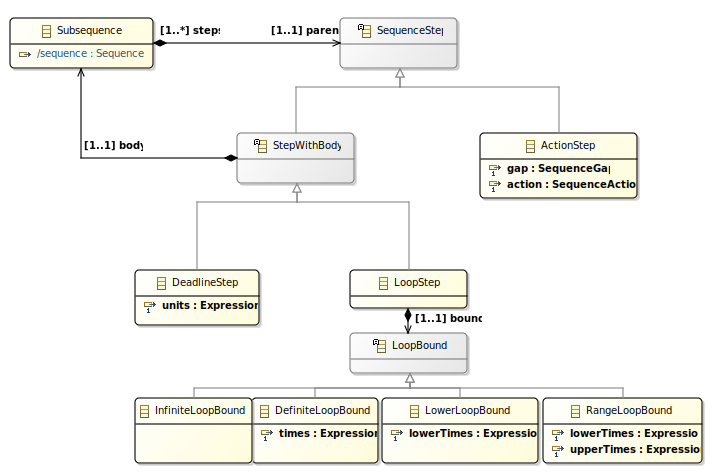
\includegraphics[width=0.7\textwidth]{diagrams/Steps}
	\caption{Class diagram for the part of the \langname{} metamodel dealing with steps.}
	\label{fig:metamodel-steps}
\end{figure}

\noindent
Steps (\msequencestep) are elements of
\msubsequence s.  They represent both communications and control flow, and
can themselves contain \msubsequence s.  There are three types of
step:

\begin{itemize}
\item \mdeadlinestep{} (\cref{ssec:metamodel-steps-deadlines});
\item \mloopstep{} (\cref{ssec:metamodel-steps-loops});
\item \mactionstep{} (\cref{ssec:metamodel-steps-actions});
\end{itemize}

\Cref{fig:metamodel-actions} depicts the part of the metamodel concerning
sequence steps.

\subsection{\mdeadlinestep}\label{ssec:metamodel-steps-deadlines}

A \mdeadlinestep{} asserts that a \msubsequence{} takes at most
a given number of time units to complete.
It takes a name (currently only
used in the graphical notation), and an expression that must
evaluate to a natural number of time units.

\begin{remark}
To specify that all actions in a \msubsequence{} must occur
immediately, use a deadline of \(0\).
\end{remark}

\begin{figure}[H]
\begin{subfigure}[t]{\egtextwidth}
\begin{lstlisting}[style=Example]
deadline T : within 3 units {
    ->op O1()
}
\end{lstlisting}
\end{subfigure}
\hfill
\begin{subfigure}[t]{\eggraphicalwidth}
  \gsecaption
  \centering
  \begin{tikzpicture}
\matrix[diagram]{
  \node[rcmodule](mstart) {\egtarget}; & \node[world](wstart) {\egworld}; \\
  & \coordinate(wds); & \\
  \coordinate(mo); & \coordinate(wo); & \\
  \coordinate(mde); & \coordinate(wde); \\
};
\draw[lifeline] (mstart) -- (mo) -- (mde);
\draw[lifeline] (wstart) -- (wds) -- (wo) -- (wde);
\gdeadline{wds}{wde}{T}{3}
\draw (mo) edge[oarrow, "O1()"] (wo);
  \end{tikzpicture}
\end{subfigure}
\end{figure}

\todo{Considering removing `deadline T :` and changing the graphical
  syntax to just contain the number of units next to the arrow, which
  I've seen rarely in some UML2 tutorials but I'm not sure if it's
  allowed in MARTE.}

\subsection{\mloopstep}\label{ssec:metamodel-steps-loops}

% Shorthand for introducing the loop action diagram matrix.
\newcommand{\egloopmatrix}{
  \node[rcmodule](mstart) {\egtarget}; \pgfmatrixnextcell \node[world](wstart) {\egworld}; \\
  \coordinate(mls); \pgfmatrixnextcell \coordinate(wls); \\
  \coordinate(mo); \pgfmatrixnextcell \coordinate(wo); \\
  \coordinate(mle); \pgfmatrixnextcell \coordinate(wle); \\
}
% Draws the entire loop diagram with the given loop bound header.
\newcommand{\egloopdiagram}[1]{
  \matrix[diagram]{\egloopmatrix};
  \draw[lifeline] (mstart) -- (mls) -- (mo) -- (mle);
  \draw[lifeline] (wstart) -- (wls) -- (wo) -- (wle);
  \draw (mo) edge[oarrow, "O1()"] (wo);
  \gloop{mls}{wls}{mle}{wle}{L}{#1}
}

A \mloopstep{} is a named loop over a \msubsequence{} of steps.
The number of times a \mloopstep{} will iterate \todo{adding breaks will
change this}
depends on its attached \mloopbound{}.  Each bound is in terms of
\mexpression{}s that are evaluated \emph{only once}, before the execution
of the loop.

\paragraph{\minfiniteloopbound}
A \minfiniteloopbound{} states that the loop executes an infinite
number of times.

\begin{figure}[H]
\begin{subfigure}[t]{\egtextwidth}
\begin{lstlisting}[style=Example]
loop L : forever { // or 'loop L {'
    ->op O1()
}
\end{lstlisting}
\end{subfigure}
\hfill
\begin{subfigure}[t]{\eggraphicalwidth}
  \gsecaption
  \centering
  \begin{tikzpicture}
    \egloopdiagram{\gloopinfinite}
  \end{tikzpicture}
\end{subfigure}
\end{figure}

\paragraph{\mdefiniteloopbound}
A \mdefiniteloopbound{} states that the loop executes exactly the
number of times given in the bound.

\begin{figure}[H]
\begin{subfigure}[t]{\egtextwidth}
\begin{lstlisting}[style=Example]
loop L : exactly 4 times {
    ->op O1()
}
\end{lstlisting}
\end{subfigure}
\hfill
\begin{subfigure}[t]{\eggraphicalwidth}
  \gsecaption
  \centering
  \begin{tikzpicture}
    \egloopdiagram{\gloopdefinite{4}}
  \end{tikzpicture}
\end{subfigure}
\end{figure}

\paragraph{\mlowerloopbound}
A \mlowerloopbound{} states that the loop executes at least the
number of times given in the bound, but may nondeterministically
choose to execute any number of times in addition.

\begin{figure}[h!]
\begin{subfigure}[t]{\egtextwidth}
\begin{lstlisting}[style=Example]
loop L : at least 5 times {
    ->op O1()
}
\end{lstlisting}
\end{subfigure}
\hfill
\begin{subfigure}[t]{\eggraphicalwidth}
  \gsecaption
  \centering
  \begin{tikzpicture}
    \egloopdiagram{\glooplower{5}}
  \end{tikzpicture}
\end{subfigure}
\end{figure}

\paragraph{\mrangeloopbound}
A \mrangeloopbound{} behaves as a \mlowerloopbound, but states that
the loop will not execute any more times than the given upper bound.
Note that if the bounds are the same, the semantics is equivalent
to that of a \mdefiniteloopbound{}.

\begin{figure}[H]
\begin{subfigure}[t]{\egtextwidth}
\begin{lstlisting}[style=Example]
loop L : between 3 and 6 times {
    ->op O1()
}
\end{lstlisting}
\end{subfigure}
\hfill
\begin{subfigure}[t]{\eggraphicalwidth}
  \gsecaption
  \centering
  \begin{tikzpicture}
    \egloopdiagram{\glooprange{3}{6}}
  \end{tikzpicture}
\end{subfigure}
\end{figure}

\subsection{\mactionstep}\label{ssec:metamodel-steps-actions}

A \mactionstep{} contains a specification of a
\msequenceaction{} (\cref{sec:metamodel-actions}), as well as
a \mmessageset{}
capturing any communications implicitly allowed to happen
in the \emph{gap} before the action.

\begin{figure}[H]
  \begin{subfigure}[c]{\egtextwidth}
    \begin{lstlisting}[style=Example]
      anything in set MS except ->op O2() until ->event E

      anything except ->op O2() until <-event E
      // shorthand for 'in {||} except ->op O2()'

      anything until ->event E
      // shorthand for 'in universe'
    \end{lstlisting}
  \end{subfigure}
  \hfill
  \begin{subfigure}[c]{\eggraphicalwidth}
    \gsecaption
    \centering
    \begin{tikzpicture}
      \matrix[diagram, column sep=15em]{
        \coordinate(m1); & \coordinate(w1); \\
        \coordinate(m2); & \coordinate(w2); \\
        \coordinate(m3); & \coordinate(w3); \\
      };
      \draw[dotted] (m1) -- (w1);
      \ggapout{m1}{\gdiff{\grefset{MS}}\gextset{\text{\lstinline[language=RoboCert]{->op O2()}}}}
      
      \draw[dotted] (m2) -- (w2);
      \ggapin{w2}{\gdiff{\guniverse}\gextset{\text{\lstinline[language=RoboCert]{->op O2()}}}}
      
      \draw[dotted] (m3) -- (w3);
      \ggapout{m3}{\guniverse}
    \end{tikzpicture}
  \end{subfigure}
\end{figure}
%%% Local Variables:
%%% mode: latex
%%% TeX-master: "../robocert"
%%% End:


\section{Actions}\label{sec:metamodel-actions}
%!TEX root=../robocert.tex
\begin{figure}
	\centering
	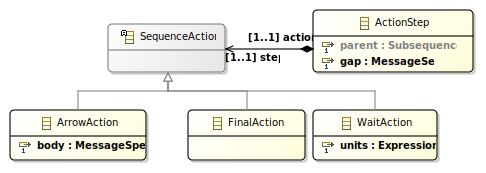
\includegraphics[width=0.7\textwidth]{diagrams/Actions}
	\caption{Class diagram for the part of the \langname{} metamodel dealing with actions.}
	\label{fig:metamodel-actions}
\end{figure}

\Cref{fig:metamodel-actions} depicts the part of the metamodel concerning
sequence actions.

A \msequenceaction{} is an explicit communication or control flow construct in a
\msubsequence.  There are currently three types of action: arrow, loop, and
final actions.

\subsection{\marrowaction}

An \marrowaction\footnote{The name signifies both that the actions resemble
PSC \emph{arrowMSG} specifications, and also that they correspond to arrows in
the graphical syntax.} specifies one communication between \mactor s which is on
the sequence specified by the diagram.  Each \marrowaction{} wraps one
\marrowmessagespec{} (\cref{sec:metamodel-messages})
containing the specification proper.
\todo{Eventually these will bind arguments.}

\begin{figure}[h!]
\begin{subfigure}[t]{\egtextwidth}
\begin{lstlisting}[style=Example]
-> operation O1()
\end{lstlisting}
\end{subfigure}
\hfill
\begin{subfigure}[t]{\eggraphicalwidth}
\gsecaption
\centering
\begin{tikzpicture}
\matrix[diagram]{
    \node[rcmodule](mstart) {\egtarget}; & \node[world](wstart) {\egworld}; \\
	\coordinate(mo); & \coordinate(wo); \\
	\coordinate(mend); & \coordinate(wend); \\
};
\draw[lifeline] (mstart) -- (mo) -- (mend);
\draw[lifeline] (wstart) -- (wo) -- (wend);
\draw (mo) edge[oarrow, "O1()"] (wo);
\end{tikzpicture}
\end{subfigure}

\end{figure}

\subsection{\mloopaction}

% Shorthand for introducing the loop action diagram matrix.
\newcommand{\egloopmatrix}{
  \node[rcmodule](mstart) {\egtarget}; \pgfmatrixnextcell \node[world](wstart) {\egworld}; \\
  \coordinate(mls); \pgfmatrixnextcell \coordinate(wls); \\
  \coordinate(mo); \pgfmatrixnextcell \coordinate(wo); \\
  \coordinate(mle); \pgfmatrixnextcell \coordinate(wle); \\
}
% Draws the entire loop diagram with the given loop bound header.
\newcommand{\egloopdiagram}[1]{
  \matrix[diagram]{\egloopmatrix};
  \draw[lifeline] (mstart) -- (mls) -- (mo) -- (mle);
  \draw[lifeline] (wstart) -- (wls) -- (wo) -- (wle);
  \draw (mo) edge[oarrow, "O1()"] (wo);
  \gloop{mls}{wls}{mle}{wle}{L}{#1}
}

A \mloopaction{} is a \emph{named} loop.  Each \mloopaction{} contains one
\msubsequence{} of steps to repeat indefinitely.

The number of times a \mloopaction{} will iterate \todo{breaking forthcoming}
depends on its attached \mloopbound{}.  Each bound is in terms of
\mexpression{}s that are evaluated \emph{only once}, before the execution
of the loop.

\paragraph{\minfiniteloopbound}
A \minfiniteloopbound{} states that the loop executes an infinite
number of times.

\begin{figure}[h!]
\begin{subfigure}[t]{\egtextwidth}
\begin{lstlisting}[style=Example]
loop L : forever { // or 'loop L {'
    -> operation O1()
}
\end{lstlisting}
\end{subfigure}
\hfill
\begin{subfigure}[t]{\eggraphicalwidth}
  \gsecaption
  \centering
  \begin{tikzpicture}
    \egloopdiagram{\gloopinfinite}
  \end{tikzpicture}
\end{subfigure}
\end{figure}

\paragraph{\mdefiniteloopbound}
A \mdefiniteloopbound{} states that the loop executes exactly the
number of times given in the bound.

\begin{figure}[h!]
\begin{subfigure}[t]{\egtextwidth}
\begin{lstlisting}[style=Example]
loop L : exactly 4 times {
    -> operation O1()
}
\end{lstlisting}
\end{subfigure}
\hfill
\begin{subfigure}[t]{\eggraphicalwidth}
  \gsecaption
  \centering
  \begin{tikzpicture}
    \egloopdiagram{\gloopdefinite{4}}
  \end{tikzpicture}
\end{subfigure}
\end{figure}

\paragraph{\mlowerloopbound}
A \mlowerloopbound{} states that the loop executes at least the
number of times given in the bound, but may nondeterministically
choose to execute any number of times in addition.

\begin{figure}[h!]
\begin{subfigure}[t]{\egtextwidth}
\begin{lstlisting}[style=Example]
loop L : at least 5 times {
    -> operation O1()
}
\end{lstlisting}
\end{subfigure}
\hfill
\begin{subfigure}[t]{\eggraphicalwidth}
  \gsecaption
  \centering
  \begin{tikzpicture}
    \egloopdiagram{\glooplower{5}}
  \end{tikzpicture}
\end{subfigure}
\end{figure}

\paragraph{\mrangeloopbound}
A \mrangeloopbound{} behaves as a \mlowerloopbound, but states that
the loop will not execute any more times than the given upper bound.
Note that if the bounds are the same, the semantics is equivalent
to that of a \mdefiniteloopbound{}.

\begin{figure}[h!]
\begin{subfigure}[t]{\egtextwidth}
\begin{lstlisting}[style=Example]
loop L : between 3 and 6 times {
    -> operation O1()
}
\end{lstlisting}
\end{subfigure}
\hfill
\begin{subfigure}[t]{\eggraphicalwidth}
  \gsecaption
  \centering
  \begin{tikzpicture}
    \egloopdiagram{\glooprange{3}{6}}
  \end{tikzpicture}
\end{subfigure}
\end{figure}

\subsection{\mfinalaction}

A \mfinalaction{} captures the successful termination of a sequence diagram.
A diagram with a \mfinalaction{} specifies a complete sequence of behaviour
from the \mtarget{} initialising to the \mtarget{} terminating.  Conversely,
sequence diagrams without \mfinalaction s capture partial specifications of
behaviour, or the behaviour of \mtarget s that do not terminate.

Note that the final \msequencegap{} before a \mfinalaction{} captures
any permitted communications after the behaviour explicitly specified by the
diagram has occurred.

\begin{figure}[h]

\begin{subfigure}[t]{\egtextwidth}
\begin{lstlisting}[style=Example]
end
\end{lstlisting}
\end{subfigure}
\hfill
\begin{subfigure}[t]{\eggraphicalwidth}
\gsecaption
\centering
\begin{tikzpicture}
\matrix[diagram]{
	\node[rcmodule](mstart) {\egtarget}; & \node[world](wstart) {\egworld}; \\
	\coordinate(mend); & \coordinate(wend); \\
};
\draw[lifeline] (mstart) -- (mend);
\draw[lifeline] (wstart) -- (wend);
\gfinal{mend}{wend}
\end{tikzpicture}
\end{subfigure}

\end{figure}

%%% Local Variables:
%%% mode: latex
%%% TeX-master: "../robocert"
%%% End:


\section{Messages}\label{sec:metamodel-messages}
%!TEX root=../robocert.tex
\begin{figure}
	\centering
	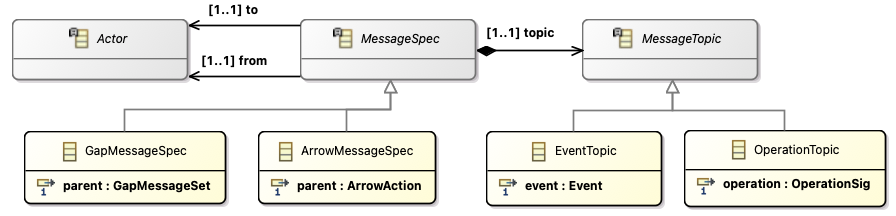
\includegraphics[width=\textwidth]{diagrams/messages.png}
	\caption{Class diagram for the part of the \langname{} metamodel dealing with messages.}
	\label{fig:metamodel-messages}
\end{figure}

\Cref{fig:metamodel-messages} depicts the part of the metamodel concerning
messages between actors.  Messages are introduced into a sequence diagram
in \mmessageset s and \marrowaction s.

\subsection{\mmessageset}\label{ssec:metamodel-messages-sets}

A \mmessageset{} is an expression of the set of messages allowed or forbidden
inside a \msequencegap.  There are two types of \mmessageset:

\begin{itemize}
\item
  a \muniversemessageset{} represents the universal set containing 
  all possible messages, and
  captures a lack of specific restriction on
  the \emph{allowed} set of a \msequencegap;
\item	
  an \mextensionalmessageset{} is a set (expressed as an unordered list) of
  zero or more \mgapmessagespec s, themselves
  a type of \mmessagespec{} (\cref{sec:metamodel-messages});
\item
  a \mrefmessageset{} refers to a \mnamedmessageset{} attached to the
  sequence.
\end{itemize}

There is not yet any meaningful extra data stored in
\mgapmessagespec s that is not present in \mmessagespec s, but this is subject
to change.

\begin{lstlisting}[style=Example]
universe                        // UniverseMessageSet
{ operation O1() from M to W }  // ExtensionalMessageSet
message set S                   // RefMessageSet
\end{lstlisting}

\subsection{\mnamedmessageset}\label{ssec:metamodel-messages-named-sets}

A \mnamedmessageset{} attaches a name to a \mmessageset, so that it can be reused
inside a \msequence.

\begin{lstlisting}[style=Example]
message set S: { operation O1() from M to W }
\end{lstlisting}

\subsection{\mmessagespec}

A \mmessagespec{} is a specification on the types of communication that can
happen during a gap (a \mgapmessagespec) or arrow (an \marrowmessagespec).\footnote{
This class distinction resembles that in PSCs betweeen intraMSGs and arrowMSGs,
respectively.}  Each \mmessagespec{} contains:

\begin{itemize}
\item
	references to two \mactor s (\cref{sec:metamodel-actors}),
	capturing the source (\emph{from}) and destination (\emph{to})
	of the communication;
\item
	the \mmessagetopic{} (\cref{ssec:metamodel-messages-topics}) specifying
	the type of communication that the spec is capturing.
\end{itemize}

\begin{figure}[h]

\begin{subfigure}[t]{0.38\textwidth}
\begin{lstlisting}[style=Example]
operation O1() from M to W
// MessageSpec with OperationTopic

event E        from W to M
// MessageSpec with EventTopic
\end{lstlisting}
\end{subfigure}
\hfill
\begin{subfigure}[t]{0.58\textwidth}
\gsecaption
\centering
\begin{tikzpicture}
\matrix[diagram]{
    \node[rcmodule](mstart) {\egtarget}; & \node[world](wstart) {\egworld}; \\
	\coordinate(mo); & \coordinate(wo); \\
	\coordinate(me); & \coordinate(we); \\
	\coordinate(mend); & \coordinate(wend); \\
};
\draw[lifeline] (wstart) -- (wo) -- (we) -- (wend);
\draw[lifeline] (mstart) -- (mo) -- (me) -- (mend);
\draw (mo) edge[oarrow, "O1()"'] (wo);
\draw (we) edge[earrow, "E"] (me);
\end{tikzpicture}
\end{subfigure}

\end{figure}

\subsection{\mmessagetopic}\label{ssec:metamodel-messages-topics}

A \mmessagetopic{} identifies the specific type of communication in a
\mmessagespec{}.  There are currently two types of topic, corresponding to
\robochart{} operations (\moperationtopic) and events (\meventtopic).
Each contains a reference to the signature of the respective construct.
Parameterised operations and events are not yet supported \todo{this will
change}.

\begin{lstlisting}[style=Example]
operation O1() // OperationTopic
event E        // EventTopic
\end{lstlisting}

\subsection{\margument}\label{ssec:metamodel-messages-arguments}

A \margument{} is a pattern that specifies (and possibly binds) one or more
arguments in
a message.  There are two types of argument:

\begin{itemize}
\item
	\mexpressionargument, which specifies that the argument is equal to the
	value of a particular \robochart{} expression;
	\todo{the CSP generator doesn't yet properly protect against this being
	an expression not expressible as a prefix}
\item
	\mrestargument, which matches \emph{all} following arguments and permits
	them to be any value.
	\todo{This mainly exists because it's very easy to specify in CSP.  Ideally
	we'll have something that allows wildcards on arbitrary parameters, in
	which case this might be confusing to have also.}
\end{itemize}

All \margument s, at time of writing, are forms of \mnonbindingargument{} and
can therefore appear in \mgapmessagespec s.  This will change when binding
arguments are introduced.

\begin{lstlisting}[style=Example]
42  // ExpressionArgument containing integer literal
... // RestArgument
\end{lstlisting}

%%% Local Variables:
%%% mode: latex
%%% TeX-master: "../robocert"
%%% End:


\section{Actors}\label{sec:metamodel-actors}
%!TEX root=../robocert.tex
\begin{figure}
	\centering
	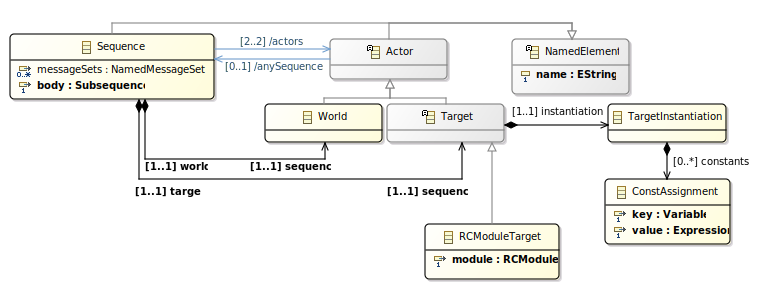
\includegraphics[width=\textwidth]{diagrams/Actors}
	\caption{Class diagram for the part of the \langname{} metamodel dealing with actors.}
	\label{fig:metamodel-actors}
\end{figure}

\Cref{fig:metamodel-actors} depicts the part of the metamodel concerning
actors.

\subsection{\mactor}

An \mactor{} is a named participant in a sequence.  The names can be used to
specify the source and recipient of communications in \mmessagespec{}s.
As mentioned in
\cref{sec:metamodel-sequences}, there are always two actors
attached to a sequence: a \mtarget{} (\cref{ssec:metamodel-actors-target})
and a \mworld{} (\cref{ssec:metamodel-actors-world}).

\subsection{\mtarget}\label{ssec:metamodel-actors-target}

A \mtarget{} references the part of a robotic system that serves as the focus
for a particular sequence diagram.  There is
presently one type of target, with more to appear later:

\begin{itemize}
\item
	a \mrcmoduletarget{} references a \mrcmodule.
\end{itemize}

All forms of \mtarget{} contain a \mtargetinstantiation{} (see below), which
is always applied to any use of that target; assertions may further instantiate
any constants left open by the target's \mtargetinstantiation.

\begin{lstlisting}[style=Example]
module M: AModule
// RCModuleTarget with implicit empty TargetInstantiation

module M: AModule
    with { SOME_CONSTANT set to 4, ANOTHER_CONSTANT set to 5 }
// RCModuleTarget with explicit TargetInstantiation
\end{lstlisting}

\subsection{\mtargetinstantiation}

A \mtargetinstantiation{} instantiates some or all of the constants in the
target's parametrisation.  It contains a list of key/value pairs where each key
is a RoboChart \mvariable{} corresponding to a constant, and each value is a
RoboChart \mexpression{} (evaluated in an empty~\todo{check this} scope).

\begin{lstlisting}[style=Example]
{ SOME_CONSTANT set to 4, ANOTHER_CONSTANT set to 5 }
\end{lstlisting}

\subsection{\mworld}\label{ssec:metamodel-actors-world}

A \mworld{} is an \mactor{} that represents the `world' outside a sequence's
\mtarget.  \mworld s do not contain any data.

\begin{lstlisting}[style=Example]
world W
\end{lstlisting}

%%% Local Variables:
%%% mode: latex
%%% TeX-master: "../robocert"
%%% End:


\section{Assertions}\label{sec:metamodel-assertions}
%!TEX root=../robocert.tex
\begin{figure}
	\centering
	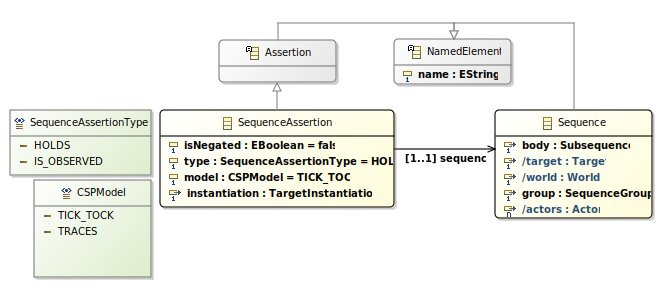
\includegraphics[width=0.7\textwidth]{diagrams/Assertions}
	\caption{Class diagram for the part of the \langname{} metamodel dealing with assertions.}
	\label{fig:metamodel-assertions}
\end{figure}

\Cref{fig:metamodel-assertions} depicts the part of the metamodel concerning
assertions.

\subsection{\massertion}

An \massertion{} is an named assertion statement.  Currently, there is
only one type of assertion: a \msequenceassertion{}.  \todo{This will change
when merging with the existing language, if not sooner.}

\subsection{\msequenceassertion}\label{ssec:metamodel-assertions-sequence}

A \msequenceassertion{} is an assertion about a particular \msequence{} with
respect to its \mtarget.  The \mtarget{} is modified by applying an
assertion-level \mtargetinstantiation, which may fix any constants not bound
by the sequence-level instantiation.  (The default is an empty instantiation,
meaning the target is exactly as specified at the sequence level.)

The specific sequence assertion type comes from the \msequenceassertiontype:
either `sequence holds on target' (refinement), or `sequence is observed on
target' (reverse refinement).  The assertion can be negated.  The choice of
\mcspmodel{} affects how the assertion is checked with CSP tools such as FDR
\todo{the models aren't actually used yet; everything is treated as untimed
traces refinement.  This will change.}

\begin{lstlisting}[style=Example]
assertion A: SequenceName holds           // positive 'holds' SequenceAssertion
assertion B: SequenceName does not hold   // negative 'holds' SequenceAssertion
assertion C: SequenceName is observed     // positive 'is observed' SequenceAssertion
assertion D: SequenceName is not observed // negative 'is observed' SequenceAssertion

assertion E: SequenceName holds with { CONSTANT set to 5 }
// example of SequenceAssertion with custom TargetInstantiation
\end{lstlisting}

%%% Local Variables:
%%% mode: latex
%%% TeX-master: "../robocert"
%%% End:


\section{Feature comparison}\label{sec:metamodel-features}
% !TEX root=../../robocert.tex
\newcommand{\insp}[1]{\ul{#1}}

This section compares \langname{} sequence features to any
corresponding features in the other notations.
For each feature, we highlight the main source of inspiration (if any)
using \insp{underlines}.

%\subsection{Sequences~(\ref{sec:metamodel-sequences})}

\subsection{Steps~(\ref{sec:metamodel-steps})}

\paragraph{\mdeadlinestep}
\begin{featset}
\item[UML] \insp{duration constraint}, time observations and constraints
\item[TPSC] clock constraint
\item[AGLPT] upper time bounds
\end{featset}

UML2 allows time and duration constraints to relate to named observations taken
previously in the sequence.  By combining a time observation at one end of a
subsequence with a time constraint at the other, we can capture a form of clock
constraint.  We do not yet capture observations.

While \robochart{} has clocks, we do not yet expose them in
\langname, as we consider them to be an implementation concern.
      
\paragraph{\mloopstep}
\begin{featset}
\item[UML] \insp{loop combined fragment}
\item[PSC] loop operator
\end{featset}

\mloopbound s are inspired by those permitted by UML.

\paragraph{Gaps}
\begin{featset}
\item[PSC] \insp{constraints}, strict operator
\item[AGLPT] until
\end{featset}

Gaps resemble past-unwanted-message constraints, but
allow restricting the set of \emph{allowed} messages;
this subsumes the strict operator.  Graphical syntax is a slight
modification of PSC syntax.  We do not cover
future-unwanted-message or chain constraints.  Currently, all
ordering is assumed strict unless modified by a gap; this
deviates from PSC \emph{and} some readings of UML.
    
\subsection{Actions~(\ref{sec:metamodel-actions})}

\paragraph{\marrowaction}
\begin{featset}
\item[UML] \insp{message occurrence specification}
\item[PSC] regular message
\end{featset}

Arrows are named for the PSC \emph{arrowMSG} concept but are closer
to UML.
      
\paragraph{\mwaitaction}
\begin{featset}
\item[UML] combination of time observations and constraints(?)
\item[TPSC] clock constraints(?)
\end{featset}

The exact form of this operator comes mostly from \robochart{} and, to
a lesser extent, \tockcsp.
Because wait actions in \langname{} assert that one
action occurs at least some time units after another, we assume that it is
possible to encode the same pattern using clock-style constraints.

\subsection{Messages~(\ref{sec:metamodel-messages})}

\paragraph{\mmessageset}
\begin{featset}
\item[PSC] \insp{constraint set}
\end{featset}

\mrefmessageset s are directly inspired by the PSC approach to referencing constraint sets.

\paragraph{\mmessagespec}
\begin{featset}
\item[UML] ??
\item[PSC] \insp{arrowMSG, intraMSG}
\end{featset}

We do not cover PSC required or fail messages.
Notion of direction (inbound/outbound) rather than sender/receiver labels.

\subsection{Actors~(\ref{sec:metamodel-actors})}

\paragraph{\mactor}
\begin{featset}
\item[UML] lifeline
\item[PSC] \insp{component instance}
\end{featset}

Unlike UML and PSC, we fix the number of actors at two
\ghtodo{32}{for now} in \langname: a \mtarget{} and a \mworld{}.
Neither are named, though the \mtarget{} will refer to a
named component such as a \mrcmodule.

Like PSC, but unlike UML, there are no executions.

\subsection{Assertions~(\ref{sec:seq-metamodel-assertions})}

As \langname{} is a notation for automated property checking,
sequence properties more closely resemble CSP-M/FDR refinement
assertions than the usual ways of reasoning about UML or PSC sequence diagrams.  As such,
features of \msequenceproperty{} capture some
concepts that are part of the diagram language 
in other notations:

\begin{itemize}
  \item
    LSC
    existential charts (specifying behaviour we expect to see at least once
    in the model) become is-observed properties in
    \langname;
  \item
    LSC notions of mandatory progress can be
    captured partially by use of tick-tock reasoning
    in \langname, though this applies to whole diagrams.
\end{itemize}

\subsection{Matrix}

\newcommand\rot{\rotatebox{90}}
\newcommand\matding[1]{{\small#1}}
\newcommand\OK{\matding{\checkmark}}
\newcommand\ASST{\matding{A}}
\newcommand\ISH{\matding{E}}
\newcommand\NO{\matding{\(\bullet\)}}
\newcommand\SOON{\matding{\(\circ\)}}
\newcommand\NA{\matding{n/a}}
\newcommand\INTIMED{\matding{T}}
\newcommand\INPROB{\matding{P}}

\begin{table}[htb!]
  \centering

  \begin{tabular}{rl|lllllll}
  \toprule

  & \rot{\thead{\langname}}
  & \rot{\thead{\featname{UML}}}
  & \rot{\thead{\featname{MARTE}}}
  & \rot{\thead{\featname{STAIRS}}}
  & \rot{\thead{\featname{LSC}}}
  & \rot{\thead{\featname{PSC}}}
  & \rot{\thead{\featname{PSP}}}
  & \rot{\thead{\featname{AGLPT}}}
  \\
  \midrule
  \multicolumn{7}{l}{\tsubhead{Modalities}}
  \\
  Universal specification
  & \OK  % Us
  & ?  % UML
  & ?  % MARTE
  & ?  % STAIRS
  & \OK  % LSC
  & ?  % PSC
  & ?  % PSP
  & ?  % AGLPT
  \\
  Existential specification
  & \ASST  % Us
  & ?  % UML
  & ?  % MARTE
  & ?  % STAIRS
  & \OK  % LSC
  & ?  % PSC
  & ?  % PSP
  & ?  % AGLPT 
  \\
  Assertion block
  & \NO  % Us
  & \OK  % UML
  & \OK  % MARTE
  & \OK  % STAIRS
  & \OK?  % LSC
  & \NO  % PSC
  & ?  % PSP
  & ?  % AGLPT 
  \\ 
  Negation block
  & \NO  % Us
  & \OK  % UML
  & \OK  % MARTE
  & \OK  % STAIRS
  & ?  % LSC
  & \NO  % PSC
  & ?  % PSP
  & ?  % AGLPT 
  \\ 
  Mandatory progress (liveness)
  & \ASST  % Us
  & ?  % UML
  & ?  % MARTE
  & ?  % STAIRS
  & \OK  % LSC
  & ?  % PSC
  & ?  % PSP
  & ?  % AGLPT 
  \\  
  \midrule
  \multicolumn{7}{l}{\tsubhead{Messages}}
  \\
  Asynchronous
  & \OK  % Us
  & \OK  % UML
  & \OK  % MARTE
  & \OK  % STAIRS
  & ?  % LSC
  & \NO  % PSC
  & ?  % PSP
  & ?  % AGLPT
  \\
  Synchronous
  & \SOON?  % Us
  & \OK  % UML
  & \OK  % MARTE
  & \OK  % STAIRS
  & ?  % LSC
  & \OK  % PSC
  & ?  % PSP
  & ?  % AGLPT
  \\
  Expected/fail
  & \NO  % Us
  & \NO  % UML
  & \NO  % MARTE
  & \NO  % STAIRS
  & \OK  % LSC
  & \OK  % PSC
  & ?  % PSP
  & ?  % AGLPT
  \\
  \midrule
  \multicolumn{7}{l}{\tsubhead{Waits}}
  \\
  Explicit (\mwaitaction)
  & \OK  % Us
  & \ISH  % UML
  & \ISH  % MARTE
  & \INTIMED  % STAIRS
  & ?  % LSC
  & \INTIMED?  % PSC
  & ?  % PSP
  & ?  % AGLPT
  \\
  Ranged
  & \SOON  % Us
  & \ISH  % UML
  & \ISH  % MARTE
  & \INTIMED  % STAIRS
  & ?  % LSC
  & \INTIMED?  % PSC
  & ?  % PSP
  & ?  % AGLPT
  \\
  \midrule
  \multicolumn{7}{l}{\tsubhead{Duration constraints}}
  \\
  Lower-bound
  & \SOON?  % Us
  & \OK  % UML
  & \OK  % MARTE
  & \INTIMED  % STAIRS
  & ?  % LSC
  & \INTIMED?  % PSC
  & ?  % PSP
  & ?  % AGLPT
  \\
  Upper-bound/deadline
  & \OK  % Us
  & \OK  % UML
  & \OK  % MARTE
  & \INTIMED  % STAIRS
  & \OK  % LSC
  & \INTIMED  % PSC
  & ?  % PSP
  & ?  % AGLPT
  \\
  \midrule
  \multicolumn{7}{l}{\tsubhead{Conditionally executed blocks}}
  \\
  Optional (\texttt{opt})
  & \SOON?  % Us
  & \OK  % UML
  & \OK  % MARTE
  & \OK  % STAIRS
  & ?  % LSC
  & \ISH  % PSC
  & ?  % PSP
  & ?  % AGLPT
  \\
  Probabilistic optional
  & \SOON  % Us
  & \NO  % UML
  & \NO  % MARTE
  & \NO  % STAIRS
  & ?  % LSC
  & \INPROB  % PSC
  & ?  % PSP
  & ?  % AGLPT
  \\
  Potential alternative (\texttt{alt}, \(\sqcap\))
  & \SOON  % Us
  & \OK  % UML
  & \OK  % MARTE
  & \OK  % STAIRS
  & ?  % LSC
  & \OK  % PSC
  & ?  % PSP
  & ?  % AGLPT
  \\
  Mandatory alternative (\texttt{xalt}, \(\extchoice\))
  & \SOON?  % Us
  & \NO  % UML
  & \NO  % MARTE
  & \OK  % STAIRS
  & ?  % LSC
  & \OK  % PSC
  & ?  % PSP
  & ?  % AGLPT
  \\
  Probabilistic alternative (\texttt{palt})
  & \SOON?  % Us
  & \NO  % UML
  & \NO  % MARTE
  & \INPROB  % STAIRS
  & ?  % LSC
  & ?  % PSC
  & ?  % PSP
  & ?  % AGLPT
  \\
  \midrule
  \multicolumn{7}{l}{\tsubhead{Other}}
  \\
  Gaps (or similar)
  & \OK  % Us
  & \NO  % UML
  & \NO  % MARTE
  & \NO  % STAIRS
  & ?  % LSC
  & \OK  % PSC
  & ?  % PSP
  & \ISH?  % AGLPT
  \\
  Loops (\mloopstep)
  & \OK  % Us
  & \OK  % UML
  & \OK  % MARTE
  & \OK  % STAIRS
  & ?  % LSC
  & \OK  % PSC
  & ?  % PSP
  & ?  % AGLPT
  \\
  Breaks
  & \SOON  % Us
  & \OK  % UML
  & \OK  % MARTE
  & \OK  % STAIRS
  & ?  % LSC
  & \OK  % PSC
  & ?  % PSP
  & ?  % AGLPT
  \\
  \bottomrule
  \end{tabular}
  \caption{Matrix of features available in \langname{} sequences compared to
  other notations.}
  \label{tab:seq-comparison-features}
\end{table}

\Cref{tab:seq-comparison-features} summarises the \langname{} features listed earlier
(which may correspond to similar features in other
notations) as well as features in other notations for which \langname{} does not yet have a counterpart.
The symbols in this table have the following meaning:

\begin{description}
  \item[\OK] Directly supported.
  \item[\SOON] Not yet supported, but
  support is planned.
  \item[\NO] Not supported or planned.
  \item[\ISH] Not directly supported, but can be encoded using other
  features.
  \item[\ASST] Not directly supported in the
  diagram language, but can be encoded using the
  assertion language.  For example, \langname{} handles
  the difference between universal and existential
  quantifications in assertions.
  \item[\INTIMED] Supported, but only in timed variants of this
  notation (for example, timed STAIRS).
  \item[\INPROB] Supported, but only in
  probabilistic variants of this
  notation (for example, probabilistic PSC). 
  \item[?] No or incomplete data.
\end{description}

%%% Local Variables:
%%% mode: latex
%%% TeX-master: "../../robocert"
%%% End:


%%% Local Variables:
%%% mode: latex
%%% TeX-master: "robocert"
%%% End:
